
\chapter{Introduction}
\label{sec:org961b6e3}
\section{Motivation}
\label{sec:orgb5c1163}

\begin{figure}[htbp]
\centering
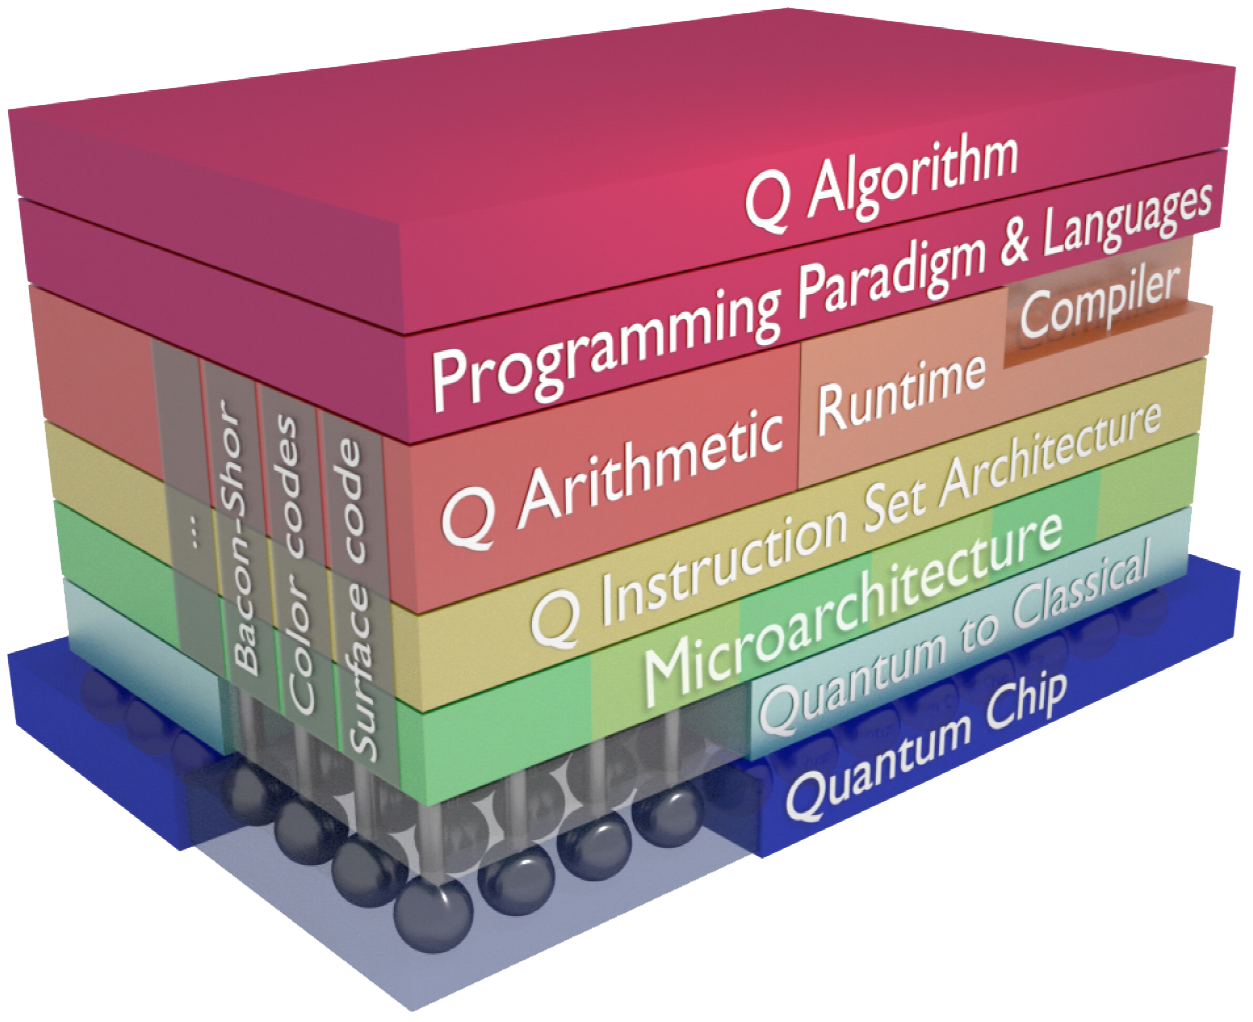
\includegraphics[width=0.7\textwidth]{figures/system_stack.png}
\caption{\label{fig:orgecea1a1}
Full stack implementation}
\end{figure}

\section{Problem Statement}
\label{sec:orgd35490c}

Quantum algorithms are represented as quantum circuits.
This notation is hardware agnostic.
Mapping models are required to have a version of the quantum algorithm adapted to the quantum device and, therefor, executable in that device.
This mapping process increases the probability of getting errors in the run of a given device, making the algorithm's results too noisy to be used.
Therefore, mapping models require an optimization process in search of the best circuit version that is executable in a given device.
Most of the works done about the mapping task optimize in terms of two parameters, either the number of added operations in the adapted version of the circuit or the latency added to the circuit.
Moreover, these works asses the quality of their mapping algorithms in one of those two metrics.
But, the information given by any of the two is enough to certify the quality of a mapping algorithm.
Given this panorama, the aim of this thesis is to study metrics to asses the quality of a mapper of quantum algorithms.

\section{Structure of the thesis}
\label{sec:org2a9c2ee}
